%!TEX root = ../thesis.tex

\section{Information Flow Control}
\label{sec:ifc}

With an architecture implemented in nuXmv, the only thing left to specify information flow properties about this architecture or its model respectively is to define how information is tracked in the model.
The general idea of information flow tracking will be adopted from \cite{Ferraiuolo17} which has been presented in section \ref{sec:bg-ifc}.
To recapture, \citeauthor{Ferraiuolo17} define three concepts:
\begin{itemize}
    \item An information flow policy in form of a lattice of security labels
    \item Information flow tracking via type-system rules
    \item Information flow control by type-checking
\end{itemize}

The information flow policy will be adopted directly.
However, since the model checker is meant to perform the information flow tracking and control, the idea of using type-checking to implement it can not be adopted directly as well.
In this section, it will be discussed how information flow tracking was lifted to the architectural level and implemented in nuXmv.

In section \ref{sec:ifc-model}, we will adopt the type system rules to instructions of the MINRV8 architecture.
Section \ref{sec:ifc-implementation} then explains how information was tracked in nuXmv.
Finally, in section \ref{sec:ifc-properties} the information flow properties that constitute the information flow control itself will be given.

\subsection{Information Flow Semantics for Instructions}
\label{sec:ifc-model}

In order to apply aforementioned type system rules of \cite{Ferraiuolo17} to instructions, the idea behind each rule will be investigated next to generate information flow semantics for instructions from those.
An interpretation function $ \I $ is introduced that maps each instruction to its information flow semantics.
We will give the semantics for instruction as functions.
These functions receive the input to the instruction as arguments and map these to the new security labels generated by the instruction.
Such input values are abstract entities.
We denote the integer value of some input $ x $ by $ v(x) \in \mathbb{Z} $ and its security labeling by $ l(x) $, i.e. $ x $ must be understood as an abstract entity.
The security labels in the architecture are tracked bitwise as words of length 8 over the alphabet $ \Sigma = \{ \PT, \PU, \CT, \CU \} $, i.e. $ l(x) \in \Sigma^8 $.
$ \bot $ refers to the least element of $ \Sigma $ in regard to $ \sqcup $, i.e. $ \bot = \PT $.

\begin{example}
    The \minrv{Sll} instruction receives two arguments: the word to shift (\texttt{rs1}) and the word indicating the amount to shift the former by (\texttt{rs2}).
    It assigns the result of this operation to some register.
    The security labeling associated with the result of \minrv{Sll} is denoted by:
    \begin{equation*}
        \I(\textsc{Sll})(\texttt{rs1}, \texttt{rs2})
    \end{equation*}

    Note, that $ \I $ does not hold semantics for \textit{where} information will flow; $ \I $ solely determines \textit{how} information flows, i.e. how labels change.
\end{example}

As we will be working with formal words, we will introduce some definitions to work with these first.
For $ w  \in \Sigma^* $, $ |w| $ denotes its length,
$ \cdot $ is used as word concatenation with its generalization over indices $ \prod $, and $ \times $ is the repeated concatenation of a word.
As we try to stay close to bit vectors, words of security labels are zero indexed and sliced from right to left, i.e. $ abcd[0] = d $ and $ abcd[1:0] = cd $.

\begin{example}
    Let $ w = abcd \in \Sigma^* $.
    \begin{itemize}
        \item $ ab \cdot cd = abcd $
        \item $ \prod_{i \in (|w|, 0]} w[i:0] = abcd \cdot abc \cdot ab \cdot a $
        \item $ 3 \times abc = abc \cdot abc \cdot abc $
    \end{itemize}
\end{example}

Furthermore, we introduce $ \ll : \Sigma^8 \times \mathbb{Z} \rightarrow \Sigma^8 $ as well as $ \gg : \Sigma^8 \times \mathbb{Z} \rightarrow \Sigma^8 $ as bit shift counterparts for words; these word shift operators are recursively defined on $ \Sigma $ as follows:

Let $ w \in \Sigma^8 $ and $ w', w'' \in \Sigma^* $ such that $ a \cdot w' = a \cdot w'' \cdot a' = w $ and $ 1 < n $.
\begin{align*}
    (a \cdot w') \ll 1 &= w' \cdot \bot \\
    w \ll n &= (w \ll 1) \ll (n - 1)
\end{align*}
\begin{align*}
    (a \cdot w'' \cdot a') \gg 1 &= a \cdot a \cdot w'' \\
    w \gg n &= (w \gg 1) \gg (n - 1)
\end{align*}

To extend this definition for shifts by amounts in $ \mathbb{Z} $ we say that $ w \ll 0 = w \gg 0 = w $ and:

Let $ n < 0 $.
\begin{align*}
    w \ll n &= w \gg |n| \\
    w \gg n &= w \ll |n|
\end{align*}

As you can see, the left shift behaves as to be expected and shifts in the least element of $ \Sigma $.
For actual bit vectors this would be the 0.
The right shift operation on the other hand does a sign extension because MINRV8 knows signed words only.

\begin{example}
    Let $ w \in \Sigma^5 $.

    \begin{align*}
        \PT \cdot \PU \cdot w \cdot \CT \ll 2 &= \PU \cdot w \cdot \CT \cdot \bot \ll 1 \\
        &= w \cdot \CT \cdot \bot \cdot \bot \\
        &= w \cdot \CT \cdot \PT \cdot \PT
    \end{align*}
    \begin{align*}
        \CU \cdot w \cdot \PU \cdot \CT \gg 2 &= \CU \cdot \CU \cdot w \cdot \PU \gg 1 \\
        &= \CU \cdot \CU \cdot \CU \cdot w
    \end{align*}
\end{example}

At last, the $ \sqcup $-supremum operator on $ \Sigma $ is extended to $ \Sigma^* $ by applying it literal-wise to a word, e.g. $ ab \sqcup cd = (a \sqcup c) \cdot (b \sqcup d) $.

With these tools at hand the translation of type system rules to semantic functions will now be presented.
Recall that MINRV8 offers 15 instructions.
For many instructions, there are type system rules that can be mapped directly.
E.g. there is no semantic difference between the \minrv{Add} instruction and performing addition in code.
However, there are some instructions that have no corresponding type-system rule in \cite{Ferraiuolo17}.
A overview of this mapping is given in table \ref{tbl:instr-mapping}.

\begin{table}
    \centering
    \begin{tabular}{| c | c |}
        \hline
        \minrv{Load} & \multirow{3}{*}{\ding{53}} \\
        \cline{1-1}
        \minrv{Store} & \\
        \cline{1-1}
        \minrv{Loadi} & \\
        \hline
        \minrv{Add} & \multirow{2}{*}{T-Arith} \\
        \cline{1-1}
        \minrv{Sub} & \\
        \hline
        \minrv{And} & \multirow{2}{*}{T-Logical} \\
        \cline{1-1}
        \minrv{Or} & \\
        \hline
        \minrv{Mov} & \ding{53} \\
        \hline
        \minrv{Sll} & T-LShift \\
        \hline
        \minrv{Sra} & T-RShift \\
        \hline
        \minrv{Ecall} & \multirow{4}{*}{\ding{53}} \\
        \cline{1-1}
        \minrv{Mret} & \\
        \cline{1-1}
        \minrv{Csrrs} & \\
        \cline{1-1}
        \minrv{Csrrc} & \\
        \hline
    \end{tabular}

    {\small \ding{53} = no mapping}
    \caption{Instruction to type system rule mapping}
    \label{tbl:instr-mapping}
\end{table}

Where an respective type system rule was assigned to an instruction, it should be obvious that the instruction actually resembles the type system rule.
For all remaining instructions, consider the list of unused type system rules in \cite{Ferraiuolo17}: T-Const (for constant expressions), T-Var (lifting types of variables), T-Concat (for bit vector concatenation) and T-ArrIndex (for array indexing).
It is obvious that most unmapped instruction in table \ref{tbl:instr-mapping} can be mapped any of the rules just listed.
The only exception to this is the \minrv{Mov} instruction the information flow of which might be specified by the T-Var rule.
However, this rule does not type variable assignments which might be of interest but variables itself.

In the following paragraphs, the information flow semantics of those instructions that have a corresponding type system rule will be given.
After that, the semantics for all remaining instructions will be discussed.
It will turn out that although there are no type system rules to derive the semantics from, the information flow associated to these instructions is rather simple and therefore can be given directly.

Firstly, the type system rule T-Logical formalizing the information flow of logical operators shall be translated.
This rule infers the type $ \tau $ of the expressions $ e_1 \land e_2 $ and $ e_1 \lor e_2 $ when $ e_1 $ and $ e_2 $ are of type $ \tau_1 $ and $ \tau_2 $ respectively by mapping each bit of the resulting word to the supremum of the labels of the argument words.
This is intuitive as for $ \land $ and $ \lor $ each bit can only be influenced by the two bits of the same index in the argument words.
This leads us to the following semantical function of \minrv{And} and \minrv{Or}:
\begin{equation*}
    \I(\textsc{And}) = \I(\textsc{Or}) = (w, w') \mapsto l(w) \sqcup l(w')
\end{equation*}

The translation of the T-Arith rule which will apply to the interpretation of the instructions \minrv{Add} and \minrv{Sub} is analogously straight-forward.
In this case, the inferred type $ \tau $ of $ e_1 + e_2 $ and $ e_1 - e_2 $ is defined as:
\begin{equation*}
    \tau = i \mapsto \bigsqcup_{j \in [1, i]} (\tau_1(j) \sqcup \tau_2(j))
\end{equation*}

Although \cite{Ferraiuolo17} not explicitly mentions whether bit vectors are one- or zero-indexed, it can be assumed for them to be one-indexed as the authors write: \textcquote{Ferraiuolo17}{%
    The rule T-Arith must track the bits that are propagated by carry bits.
    The $ i^\textit{th} $ bit of the result is affected by all bits below $ i $ from both inputs.%
}
As the definition of $ \tau $ uses indexing over the set $ [ 1, i ] $ it can be assumed for bit vectors to be one indexed as the alternative, i.e. zero-indexing, would contradict each bit being affected by \enquote{all bits below} - the definition would skip bit zero.

The label of each bit of the result is inferred by taking the supremum of all bits that come below in order to deal with possible carrying of bits.
This leads to a partially ordered sequence of security labels, i.e. we have $ \forall i' > i. \tau(i) \succeq \tau(i') $ where $ \preceq $ denotes the partial order on $ \Sigma $ induced by $ \sqcup $.
This notion is adopted to words of labels by the helper function extendSup which is defined as follows:
\begin{equation*}
    \text{extendSup} = x \mapsto \prod_{i \in (|x|, 0]} \Big( \bigsqcup_{j \in [0, i]} x[j] \Big)
\end{equation*}

extendSup implements the idea of the mapping $ \tau $ from the rule T-Arith and subsequently \textit{extends} the label of each index $ i $ to all indices greater than $ i $ which map to a $ \preceq $-smaller label.

\begin{example}
    \begin{equation*}
        \text{extendSup}(\CU \cdot
        \PU \cdot \PT) = \CU \cdot \PU \cdot \PT
    \end{equation*}

    \begin{equation*}
        \text{extendSup}(\PU \cdot \CU \cdot \PU \cdot \PT \cdot \PU) = \CU \cdot \CU \cdot \PU \cdot \PU \cdot \PU
    \end{equation*}
\end{example}

With extendSup, the semantics of the \minrv{Add} and \minrv{Sub} instructions can be defined.
\begin{equation*}
    \I(\textsc{Add}) = \I(\textsc{Sub}) = (w, w') \mapsto \text{extendSup}\big(l(w) \sqcup l(w') \big)
\end{equation*}

\begin{example}
    Consider the addition of two bit vectors which generally are considered to be public and untrusted with one bit being confidential and trusted.
    \begin{align*}
        & \I(\textsc{Add})(\PU \cdot \CT \cdot \PU, \PU \cdot \PU \cdot \PU) \\
        =& \text{extendSup}((\PU \cdot \CT \cdot \PU) \sqcup (\PU \cdot \PU \cdot \PU)) \\
        =& \text{extendSup}(\PU \cdot \CU \cdot \PU) \\
        =& \CU \cdot \CU \cdot \PU
    \end{align*}
\end{example}

T-LShift and T-RShift infer the type of $ e \ll n $ and $ e \gg n $ by simply shifting the labels.
The biggest part of these type system rules has already been translated in the definition of $ \ll $ and $ \gg $ on security label words with the only difference being that shifts in SecVerilogBL are unsigned.
Therefore in the type system rules, $ \bot $ is shifted in not only for left shifts but also for right shifts; this exception has been already coped with in the definition of $ \gg $.

However, in \cite{Ferraiuolo17} the authors also only know one source of labels, i.e. the word that is shifted, because shifts can only occur by constant amounts\footnote{%
    Recall that constants in SecVerilogBL are of type $ \bot $, i.e. do not need to be considered further as $ x \sqcup \bot = x $.
}.
In the context of this thesis, the value of a register determines the amount a word will be shifted by, i.e. that amount is dynamic and has its own security labels.
We therefore extend the interpretation of the \minrv{Sll} and \minrv{Sra} instructions by taking the maximum label of the amount the word will be shifted by and applying this label to all labels of the shifted word.
The reasoning behind this is that each bit of the word shifted is influenced by the amount it will be shifted by.
\begin{align*}
    \I(\textsc{Sll}) &= (w, s) \mapsto \big(l(w) \ll v(s) \big) \sqcup \Big(|l(s)| \times \bigsqcup l(s) \Big) \\
    \I(\textsc{Sra}) &= (w, s) \mapsto \big(l(w) \gg v(s) \big) \sqcup \Big(|l(s)| \times \bigsqcup l(s) \Big)
\end{align*}

Now, the only thing left is to give semantics for all the instruction that do not have an analogous type system rule, i.e. \minrv{Slt}, \minrv{Mov}, \minrv{Load}, \minrv{Store}, \minrv{Csrrs} and \minrv{Csrrc}, \minrv{Loadi}.

\minrv{Slt} sets only one bit of the targeted register thus its semantics also should set only one literal of the resulting security labeling.
As all bits are taken into account when comparing two bit vectors, the resulting bit is set to the maximum of all bits of both arguments.
\begin{equation*}
    \I(\textsc{Slt}) = (w, w') \mapsto (7 \times \bot) \cdot \Big(\bigsqcup l(w) \sqcup \bigsqcup l(w') \Big)
\end{equation*}

The semantics of \minrv{Mov} is rather simple.
Since \minrv{Mov} only \textit{moves} information, the labels of a moved word must not change:
\begin{equation*}
    \I(\textsc{Mov}) = w \mapsto l(w)
\end{equation*}

Similar is true for \minrv{Load} and \minrv{Store}.
These instructions also simply move values through the architecture and therefore also simply cascade security labels.
However, as memory addressing is dynamic via indices stored in registers the labels to propagate for a read are not associated with the inputs to the instruction itself but with the memory location that is read.
The magic function \mbox{memoryLabel} that maps memory addresses to the corresponding labelings copes with this.
It allows to define the semantics of \minrv{Load} and \minrv{Store} as follows:
\begin{align*}
    \I(\textsc{Load}) &= a \mapsto \text{memoryLabel}\big(v(a) \big) \\
    \I(\textsc{Store}) &= (a, d) \mapsto l(d)
\end{align*}

A similar magic function is needed for the semantics of \minrv{Csrrs} and \minrv{Csrrc}.
The magic function \mbox{csrLabel} that maps \gls{csr}-indices to the corresponding security labelings deals with \gls{csr} reads as these happen via index as well.
\begin{align*}
    \I(\textsc{Csrrs}) = \I(\textsc{Csrrc}) &= (r, w) \mapsto \text{csrLabel}\big(v(r) \big)
\end{align*}

Finally, the semantics of \minrv{Loadi} is coupled to the current execution context.
Under the given threat-scenario (cf. section \ref{sec:threat-model}), it is sensible to assume that constants loaded by machine-mode are always labelled with \CT{} and constants loaded by user-mode are always labeled with \PU{}.
\begin{equation*}
    \I(\textsc{Loadi}) = c \mapsto \begin{cases}
        8 \times \CT & \; \text{if current mode is machine-mode} \\
        8 \times \PU & \; \text{if current mode is user-mode}
    \end{cases}
\end{equation*}

\paragraph{Summary}
A final overview of all information flow semantics for instructions that have been introduced in this section can be found in figure \ref{fig:ifc-semantics}.
Note that not all labels of all inputs are used when generating new labelings; these include\footnote{%
    The label of $ c $ for \minrv{Loadi} is also not being used but in this case, the constant $ c $ does not have a label assigned as it is not a proper value of the architecture.
    This is not made explicit by our formalisms as they don't differentiate between such \textit{proper values} and hard-coded constants but is inline with the type system rules in \cite{Ferraiuolo17}.
}:
\begin{itemize}
    \item The label of the address register $ a $ for the \minrv{Load} and \minrv{Store} instructions
    \item The label of the \gls{csr}-write register $ w $ for the \minrv{Csrrs} and \minrv{Csrrc} instructions
\end{itemize}

The labels of these values have been left untouched purposefully.
This does not mean that these labels don't matter to the system as a whole.
However, they don't constitute the new labels of the actual \textit{values} moved through the architecture.
The labels of these values will be used by the properties the architecture will be verified against.
More on this in section \ref{sec:ifc-properties}.

\begin{figure}
    \begin{align*}
        \text{extendSup} &= x \mapsto \prod_{i \in (|x|, 0]} \Big( \bigsqcup_{j \in [0, i]} x[j] \Big) \\
        \I(\textsc{And}) &= \I(\textsc{Or}) = (w, w') \mapsto l(w) \sqcup l(w') \\
        \I(\textsc{Add}) = \I(\textsc{Sub}) &= (w, w') \mapsto \text{extendSup}\big(l(w) \sqcup l(w') \big) \\
        \I(\textsc{Sll}) &= (w, s) \mapsto \big(l(w) \ll v(s) \big) \sqcup \Big(|l(s)| \times \bigsqcup l(s) \Big) \\
        \I(\textsc{Sra}) &= (w, s) \mapsto \big(l(w) \gg v(s) \big) \sqcup \Big(|l(s)| \times \bigsqcup l(s) \Big) \\
        \I(\textsc{Slt}) &= (w, w') \mapsto \bot\bot\bot\bot\bot\bot\bot \cdot \Big(\bigsqcup l(w) \sqcup \bigsqcup l(w') \Big) \\
        \I(\textsc{Mov}) &= w \mapsto l(w) \\
        \I(\textsc{Load}) &= a \mapsto \text{memoryLabel}\big(v(a) \big) \\
        \I(\textsc{Store}) &= (a, d) \mapsto l(d) \\
        \I(\textsc{Csrrs}) = \I(\textsc{Csrrc}) &= (r, w) \mapsto \text{csrLabel}\big(v(r) \big) \\
        \I(\textsc{Loadi}) &= c \mapsto \begin{cases}
            8 \times \CT & \; \text{if current mode is machine-mode} \\
            8 \times \PU & \; \text{if current mode is user-mode}
        \end{cases}
    \end{align*}
    \caption{Information flow semantics for instructions}
    \label{fig:ifc-semantics}
\end{figure}

\subsection{Implementation of Information Flow Tracking}
\label{sec:ifc-implementation}

In order to implement the information flow tracking semantics described in section \ref{sec:ifc-model} we define a binary representation of the lattice of security labels given by $ \Sigma $ and $ \sqcup $.
Let $ \binSigma = \{ 00, 01, 10, 11 \}$ with a mapping $ \varphi : \Sigma \rightarrow \binSigma $ such that:
\begin{align*}
    \varphi(\PT) &= 01 \\
    \varphi(\PU) &= 00 \\
    \varphi(\CT) &= 11 \\
    \varphi(\CU) &= 10
\end{align*}

\begin{figure}
    \centering
    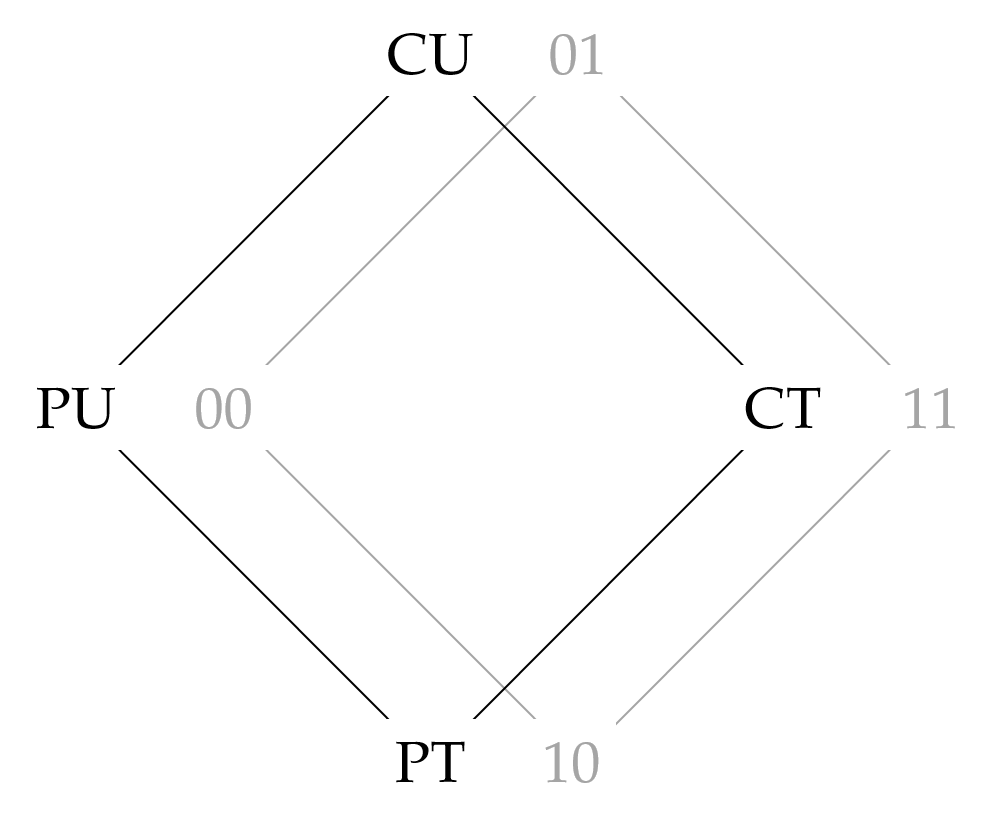
\includegraphics[width=0.4\textwidth]{figures/binary-lattice.png}
    \caption{Security lattice for SecVerilogBL \cite{Ferraiuolo17} with binary equivalent}
    \label{fig:sec-lattice-bin}
\end{figure}

Let $ \sqcup $ be defined on $ \binSigma $ such that $ \varphi $ is an isomorphism, e.g. $ 00 \; \sqcup \; 11 = 10 $.
This mapping is depicted in figure \ref{fig:sec-lattice-bin}.
Note that public and untrusted correspond to a 0 whereas confidential and trusted correspond to a 1.
This abstraction can be formalized by examining two equivalence-relations or -classes on $ \Sigma $ and $ \binSigma $.
We define two partitionings $ \Sigma/_{\equiv_C} $ and $ \Sigma/_{\equiv_I} $ on $ \Sigma $ which induce corresponding equivalence classes of security labels modulo confidentiality $ \equiv_C $ or modulo integrity respectively $ \equiv_I $.
\begin{align*}
    \Sigma /_{\equiv_C} &= \big\{ \{ \PU, \PT \}, \{ \CU, \CT \} \big\} \\
    \Sigma /_{\equiv_I} &= \big\{ \{ \PU, \CU \}, \{ \PT, \CT \} \big\}
\end{align*}

We coin the names $ \P = [\PU]_{\equiv_C} $, $ \C = [\CU]_{\equiv_C} $, $ \U = [\PU]_{\equiv_I} $ and $ \T = [\PT]_{\equiv_I} $ and lift $ \sqcup $ to be defined on equivalence-classes in the usual fashion, i.e. $ [x] \sqcup [y] = [x \sqcup y] $.
Note that this allows lifting of the $ \preceq $ order on $ \Sigma $ as well, i.e. $ \P \preceq \C $ and $ \T \preceq \U $ where $ \P \preceq \C $ iff there is no label $ l_1 \in \C $ such that for any $ l_2 in \P $ one has $ l l_1 \preceq l_2 $, and that all labels can be represented by the intersection of the respective equivalence classes,i.e. $ \{ \PU \} = \P \cap \U $.
Furthermore, it is possible to define $ \sqcup $ solely by working with these equivalence classes:
\begin{equation*}
    \{ x \sqcup y \} = \big(([x]_{\equiv_C} \sqcup [y]_{\equiv_C}) \cap ([x]_{\equiv_I} \sqcup [y]_{\equiv_I}) \big)
\end{equation*}

\begin{example}
    \begin{align*}
        \{ \PU \sqcup \CT \} &= \big(([\PU]_{\equiv_C} \sqcup [\CT]_{\equiv_C}) \cap ([\PU]_{\equiv_I} \sqcup [\CT]_{\equiv_I}) \big) \\
        &= \big((\P \sqcup \C) \cap (\U \sqcup \T) \big) \\
        &= (\C \cap \U) \\
        &= \{ \CU \}
    \end{align*}
\end{example}

This means that labels of the lattice $ (\Sigma, \sqcup, \sqcap) $ can be tracked by considering the confidentiality and integrity parts individually.
In other words: in general one can calculate the supremum or infimum of two labels by performing the respective operation on the parts in the domains of confidentiality and integrity individually.
This is illustrated in figure \ref{fig:lattice-equiv-classes} where again the lattice of security labels is shown but there also are two axes which divide each domain in half.
There, you can see why, e.g. $ \{ \PT \} = \P \cap \T $ and also that $ \P \sqcup \C = \C $ or $ \T \sqcup \U = \U $.

\begin{figure}
    \centering
    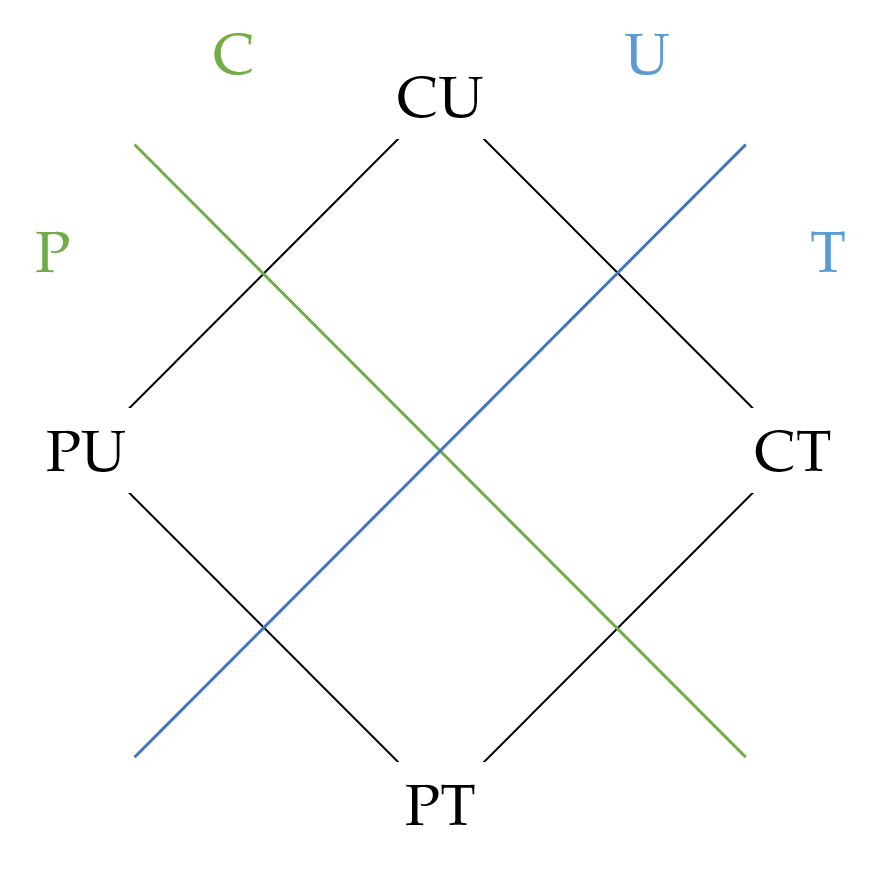
\includegraphics[width=0.4\textwidth]{figures/equivalence-class-lattice.png}
    \caption{Security lattice for SecVerilogBL \cite{Ferraiuolo17} with equivalence-classes}
    \label{fig:lattice-equiv-classes}
\end{figure}

Dealing with information flow labels in this way also is much more intuitive:
\begin{itemize}
    \item Two sources of information combined are considered to be confidential if \textit{any} of the sources is confidential.
    This is sensible as with some result of an operation at least partial knowledge about its confidential source can be inferred- depending on whether the public source or the operation are known.
    \item Two sources of information combined are considered to be trustworthy if \textit{both} of the sources are trustworthy themselves.
    This is intuitive as well.
    Non-trustworthy sources of information are assumed to be controlled by an attacker.
    Some piece of information can only be trustworthy if it can be ensured that the attacker does not control it in any way, shape or form.
    This is only given if both of the sources of an operation are not controlled by an attacker, i.e. are trustworthy.
\end{itemize}

The intuition behind $ \sqcup $ as described above perfectly matches $ \binSigma $ as well.
Recall, that \C{} is represented by a 1 and \P{} by a 0 in the binary representation.
That means that two labels $ a = a_Ca_I \in \binSigma $ and $ b = b_Cb_I \in \binSigma $ are in \C{}, i.e. confidential, if $ a $ or $ b $ is confidential, i.e. if \textit{one} of the bits representing the confidentiality of the labels is high, i.e. if $ a_C \lor b_C $.
In turn, these two labels are in $ \T $, i.e. trusted, if $ a $ and $ b $ are trusted, i.e. if \textit{both} of the bits representing the integrity of the labels are high, i.e. if $ a_I \land b_I $.
This allows us to define $ \sqcup $ on $ \binSigma $ again - this time not just semantically:
\begin{equation*}
    a_C a_I \sqcup b_C b_I = (a_C \lor b_C) \cdot (a_I \land b_I)
\end{equation*}

In summary, these paragraphs showed to things:
\begin{enumerate}
    \item Information flow labels of information can be tracked by using separate labels for the domain of confidentiality and the domain of integrity which in turn can be stored independently of each other.
    This means that the implementation of the MINRV8 architecture does not need to work with the full lattice of information flow labels itself.
    It is sufficient to deal with equivalence classes which can be inferred from individual bits.
    \item The $ \sqcup $ operation on the binary representation $ \binSigma $ of the security labels can be implemented by concatenating the logical disjunction ($ \lor $) of the confidentiality bits and the logical conjunction ($ \land $) of the integrity bits.
\end{enumerate}

This now allows for adding security label tracking to the model in nuXmv.
Labels are assigned on a per bit basis to all values in registers, memory, \glspl{csr} and the cache.
For each variable in the model, an confidentiality or integrity tracking counterpart as (arrays of) unsigned word(s) is added; find an overview of all such variables in table \ref{tbl:ifc-vars}.

\begin{table}
    \centering
    \begin{tabular}{| c | c | c |}
        \hline
        \textbf{Variable} & \textbf{Confidentiality Tracking} & \textbf{Integrity Tracking} \\
        \hline
        {\smv{regs}} & {\smv{regs_conf}} & {\smv{regs_integrity}} \\
        {\smv{memory}} & {\smv{memory_conf}} & {\smv{memory_integrity}} \\
        {\smv{csrs}} & {\smv{\_\_csrs_conf}} & {\smv{\_\_csrs_integrity}} \\
        {\smv{cache.line}} & {\smv{cache.conf}} & {\smv{cache.integrity}} \\
        \hline
    \end{tabular}
    \caption{Information Flow Control Variables}
    \label{tbl:ifc-vars}
\end{table}

These variables transition under the same conditions as their base variable does, e.g. \smv{regs_conf} does a transition if and only if \smv{regs} transitions and \smv{regs_conf} will deduct its content from sources parallel the those of \smv{regs}.
The values themselves change based on the current instruction and its information flow tracking semantics as described in section \ref{sec:ifc-model}.
The only exception to this is the information flow tracking of the variable \smv{csrs} the labels of which do not change at all.
\Glspl{csr} are assigned constants labels because they do not store information but reflect the architectures state.
Certain parts of the architectural state might be for example confidential but the characteristic of being confidential is not determined by the actual value that the respective \gls{csr} is written with but the kind of state that is defined by it.

In other words, the \lstinline[language=SMV,mathescape]{$\dots$_conf} and \lstinline[language=SMV,mathescape]{$\dots$_integrity} variables mirror the architectural part of implementation as described in section \ref{sec:model-implementation}.
The domain of confidentiality and the domain of integrity of the MINRV8 architecture are tracked in addition to simulating the pure computational world where variables implementing the information flow tracking change in parallel to their counterparts in the computational world.

\subsection{Information Flow Properties}
\label{sec:ifc-properties}

Finally, the information flow properties constituting the information flow control will be defined now.
Each property is expressed as an \gls{ltl} formula of the form \smv{assumptions -> G expr}.
\smv{assumptions} here is a macro that will be replaced by a conjunction of assumptions that assume programs running on the architecture to obey the rules to secure usage of the architecture as discussed in \ref{sec:sum-background}.

In the summary of section \ref{sec:ifc-model}, it was mentioned that there are some arguments to the information flow semantic functions in $ \I $ that are not used to determine the information flow label of some architectural word.
These induce the first properties the MINRV8 architecture will be verified against.

Firstly, recall the definition of the LOAD and STORE semantics.
The new tracking labels resulting from executing such an instruction solely depend on the labels of the word loaded or stored.
What hasn't been used in the definition of information flow is the label of the target address of the memory operation.
It is intuitive that the address does not influence the label of the information itself.
This leads to the following property:
\begin{enumerate}[label=\Roman*.,series=]
    \item \label{itm:prop-mem-i}
    Whenever a memory operation is performed in privileged mode, the target address must be integrous.

    \begin{lstlisting}[
        language=smv,
        caption={Implementation of property \ref{itm:prop-mem-i}},
        label={snpt:prop-mem-i}
    ]
        LTLSPEC NAME MEMORY_OP_INTEGRITY :=
            assumptions -> G (
                priv & op in { LOAD, STORE }
                -> (regs_integrity[rs1] & 0h_03) = 0h_03
            );
    \end{lstlisting}
\end{enumerate}

Secondly, recall the definition of the semantics for \rv{Csrrs} or \rv{Csrrc}, respectively.
These only propagate information flow tracking labels by assigning the constant labels of the \gls{csr} read to the respectively targeted register.
We decided to model the labels of \glspl{csr} as constants because they control the state of the architecture and as such might be target of an attack.
We labelled all \glspl{csr} as integrous and \gls{mstatus} as confidential.
We decided to not label \gls{pmacfg} or \gls{pmpcfg} as confidential since it can be assumed that user mode must be able to know where memory regions are to operate correctly.

Coming back to the information flow semantics of \rv{Csrrs} and \rv{Csrrc}, notice that in the respective definition of the semantical functions the value the \glspl{csr} are written with is not used.
This must necessarily be the case since the labels of the \glspl{csr} are constant and as such can not change based on the labels of the value to write them with.
However, this leads us to phrase a property about the \gls{csr} labels that ensures their integrity:
\begin{enumerate}[label=\Roman*.,resume]
    \item \label{itm:prop-csr-i}
    Whenever a \gls{csr} is written, the value it is written with must be integrous.

    \begin{lstlisting}[
        language=smv,
        caption={Implementation of property \ref{itm:prop-csr-i}}
    ]
        LTLSPEC NAME CSR_INTEGRITY :=
            assumptions -> G (
                priv & op in { CSRRS, CSRRC }
                -> regs_integrity[rs2] = 0h_FF
            );
    \end{lstlisting}
\end{enumerate}

Both of these properties are founded in intuition as well.
It is not safe to have an attacker control the load and store instructions of machine-mode since this could lead to unwanted behavior of code.
One might object that this is not problematic since, if a malicious value was to be loaded by machine-mode, information flow tracking should catch this, however, this must not necessarily be the case.
An attacker could trick machine-mode into using a value that is labelled as integrous but coincidentally diverges the control flow of machine-mode in a way that is beneficial to an attacker.
Additionally, it is obvious that \glspl{csr} should only be written with trusted data.

From all the variables our implementation of the MINRV8 architecture comprises we now considered \smv{regs} and \smv{memory} as well as \smv{cache} in regards to the security of the architecture by looking at the gaps of the information flow semantic functions.
We also considered the variable \smv{csrs} by assigning constant information flow labels to it and using it as an information flow target, i.e. we phrased properties ensuring that certain flows of information \textit{to} \smv{csrs} do not occur.
However, up to this point the \smv{priv} variable which holds the current privilege mode was only handled implicitly.
It was used as a source of labels since it determines the labels of machine words loaded as immediates by LOADI.

It is reasonable to assume, though, that \smv{priv} also can serve as an information flow target - similar to \smv{csrs}.
We already did this partially for property \ref{itm:prop-mem-i} where we assumed the architecture to be in privileged mode.
These properties, however, only dealt with the integrity labels of information.
The domain of confidentiality has yet been left out so we will introduce one final property for verification that covers the interplay between privilege mode and confidentiality labels:
\begin{enumerate}[label=\Roman*.,resume]
    \item \label{itm:prop-no-leak}
    Whenever the architecture is in user mode, there is no confidential data in any register.

    \begin{lstlisting}[
        language=smv,
        caption={Implementation of property \ref{itm:prop-no-leak}},
        label={snpt:prop-no-leak}
    ]
        LTLSPEC NAME NO_LEAK :=
            assumptions -> G (priv | (
                regs_conf[0] = 0h_00
                & regs_conf[1] = 0h_00
                & regs_conf[2] = 0h_00
                & regs_conf[3] = 0h_00
            ));
    \end{lstlisting}
\end{enumerate}

\subsection{Summary}

\todo[inline]{Write}

\todo{Use graphic}
\begin{figure}
    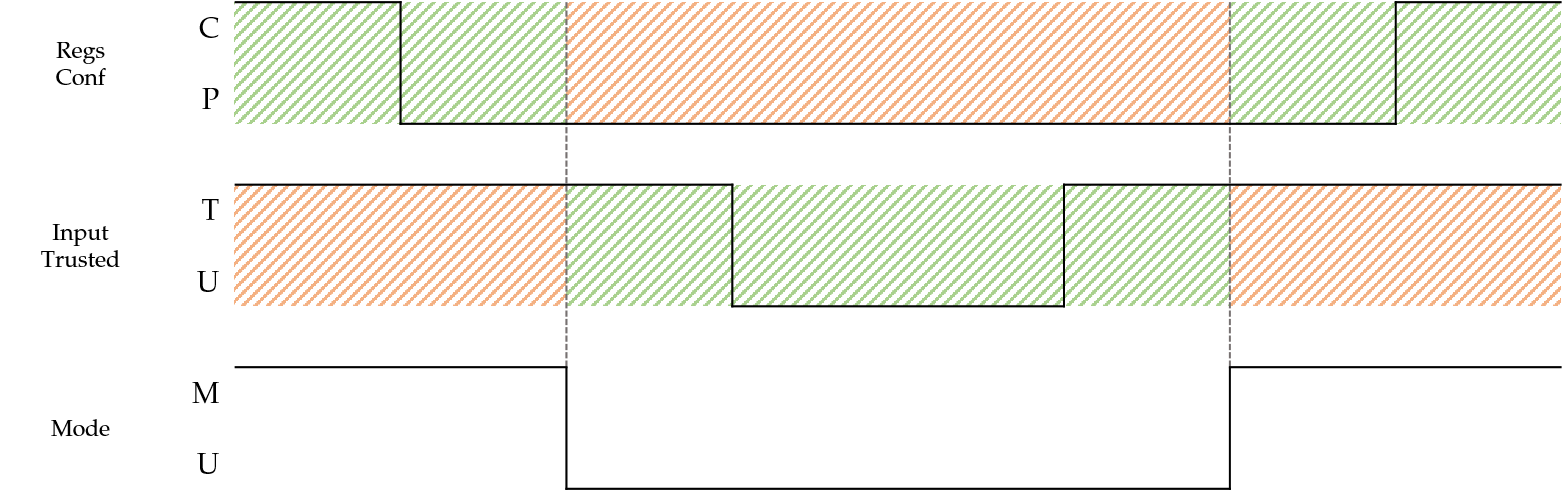
\includegraphics[width=\textwidth]{figures/properties.png}
\end{figure}
